\documentclass[journal]{IEEEtran}
\usepackage[caption=false,font=footnotesize]{subfig}
\usepackage{booktabs}
\usepackage{datatool}
\usepackage{listings}
\usepackage{makecell}
\usepackage{tikz}
\usetikzlibrary{positioning}
\usetikzlibrary{trees}
\usetikzlibrary{fit}
\usetikzlibrary{backgrounds}
\usepackage[hyphens]{url}

\lstdefinestyle{lststyle}{
	aboveskip=20pt,
	belowskip=20pt,
	frame=single,
	basicstyle=\tt\scriptsize,
	commentstyle=\color{gray}}

\begin{document}
\DTLloaddb{keys_values}{results/keys-values.csv}

\title{Reproducible Builds for Computational Research Papers}

\author{Paschalis~Bizopoulos and Dimitris~Bizopoulos
\thanks{P. Bizopoulos and D. Bizopoulos are Independent Researchers, Thessaloniki, Greece e-mail: pbizopoulos@protonmail.com, dimitrisbizopoulos@gmail.com}}

\maketitle

\begin{abstract}
	Previous work in reproducibility focused on providing frameworks to make research reproducible, however without taking in consideration the cost of extra work that needs to be done by the authors.
	We propose applying the concept of reproducible builds on computational research papers written in \LaTeX.
	The authors use a template that allows them to verify the reproducibility of their paper locally.
	The authors can share the reproducibility status of their paper with reviewers using the following procedure.
	When they push their code to their remote repository a predetermined number of docker containers are built and run in separate Virtual Machines (VMs) reproducing the figures, tables and variables (results) of the paper.
	The previous results are used during the \LaTeX\ compilation in each VM, to produce corresponding pdf files.
	Lastly another VM certifies the research paper as reproducible, if and only if the resulted pdf files are identical.
	The first builds are needed to enable comparison between different builds of the same source code and any non-deterministic stochasticity would produce different pdf files for different builds, thus making the certifier VM report the paper as non-reproducible.
	We release an open source implementation of this procedure and certify the reproducibility of this paper.
\end{abstract}

\section{Introduction}
A research paper is considered reproducible when reviewers are able to reproduce its results, given the data and experimental procedure.
More specifically, computational research reproducibility requires the presence of source code that produces or fetches data from external sources which then transforms them creating the figures, tables and variables of the paper.
Open sourcing the code and the raw data of a computational research paper helps in increasing the credibility of the research results but this is not enough to certify its reproducibility.
A common workflow among researchers for certifying computational research papers will push the direction towards creating reproducible research, thus tackling the `reproducibility crisis' problem.

We propose reproducible builds that certify the reproducibility of computational research papers written in \LaTeX.
The workflow consists of multiple separate Virtual Machines (VMs) that build and run the Docker container which produces the figures, tables, variables (results), and later compile the \LaTeX\ to produce pdf files.
Lastly, another VM compares the pdf files and certifies the research paper as reproducible, if and only if the pdf files are identical bit by bit.

We provide an implementation\footnote{\url{https://github.com/pbizopoulos/reproducible-builds-for-computational-research-papers}} of the Reconciler, that certifies the reproducibility of the arXiv version of this paper\footnote{\url{https://arxiv.org/abs/2005.12660}}.
We use Python~\cite{van2007python} for producing the results, however other scientific-oriented programming languages such as R~\cite{ihaka1996r} and Julia~\cite{bezanson2017julia} can be used.

For the rest of the paper we will refer to:
\begin{itemize}
	\item `paper' as a computational research paper,
	\item `results' as the figures, tables and variables that are shown in the paper,
	\item `\LaTeX\ code' as the files containing the main text (\textit{*.tex} files) and bibliography (\textit{*.bib} files) of the research paper,
	\item `results code' as the files containing the scientific-oriented programming language code that produces the results (\textit{*.py} files) and
	\item `code' as both the `\LaTeX\ code' and `results code'.
\end{itemize}

\section{The Reconciler Workflow}

\begin{figure*}[!t]
	\begin{minipage}{0.2\linewidth}
		\centering
		\subfloat[]{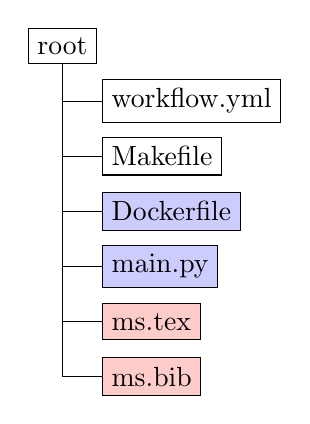
\begin{tikzpicture}[%
				grow via three points={one child at (0.5,-0.7) and
				two children at (0.5,-0.7) and (0.5,-1.4)},
				edge from parent path={(\tikzparentnode.south) |- (\tikzchildnode.west)}]
				\node[draw]{root}
				child{node[draw, anchor=west]{workflow.yml}}
				child{node[draw, anchor=west]{Makefile}}
				child{node[draw, anchor=west, fill=blue!20]{Dockerfile}}
				child{node[draw, anchor=west, fill=blue!20]{main.py}}
				child{node[draw, anchor=west, fill=red!20]{ms.tex}}
				child{node[draw, anchor=west, fill=red!20]{ms.bib}};
		\end{tikzpicture}
		\label{subfig:filehierarchy}}
	\end{minipage}
	\begin{minipage}{0.8\linewidth}
		\centering
		\subfloat[]{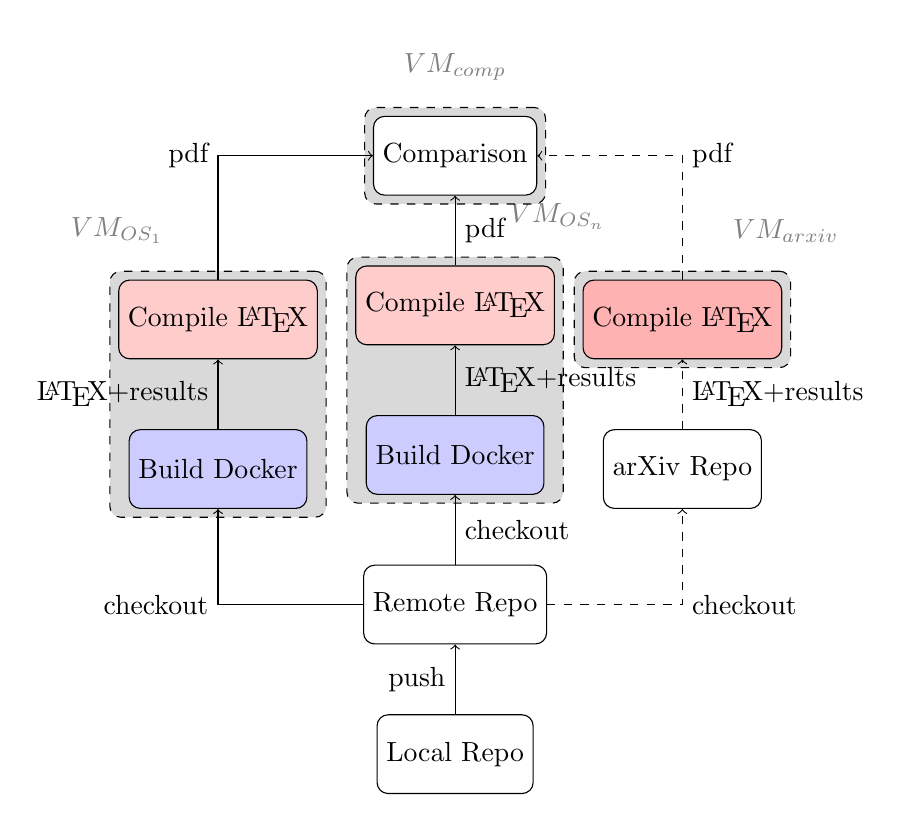
\begin{tikzpicture}[node distance=1.9cm, minimum height=1cm]
			\node[draw, rounded corners] (localrepo) {Local Repo};
			\node[draw, rounded corners, above of=localrepo] (remoterepo) {Remote Repo};
			\node[draw, rounded corners, above left=1cm of remoterepo, fill=blue!20] (builddocker1) {Build Docker};
			\node[draw, rounded corners, above of=builddocker1, fill=red!20] (compilelatex1) {Compile \LaTeX};
			\node[draw, rounded corners, above of=remoterepo, fill=blue!20] (builddocker2) {Build Docker};
			\node[draw, rounded corners, above of=builddocker2, fill=red!20] (compilelatex2) {Compile \LaTeX};
			\node[draw, rounded corners, above right=1cm of remoterepo] (arxivrepo) {arXiv Repo};
			\node[draw, rounded corners, above of=arxivrepo, fill=red!30] (compilelatex3) {Compile \LaTeX};
			\node[draw, rounded corners, above of=compilelatex2, fill=white] (comparison) {Comparison};
			\path[draw, ->] (localrepo) -- node[left]{push} (remoterepo);
			\path[draw, ->] (remoterepo) -| node[left]{checkout} (builddocker1);
			\path[draw, ->] (builddocker1) -- node[left]{\LaTeX+results}(compilelatex1);
			\path[draw, ->] (compilelatex1) |- node[left]{pdf} (comparison);
			\path[draw, ->] (remoterepo) -- node[right]{checkout} (builddocker2);
			\path[draw, ->, dashed] (remoterepo) -| node[right]{checkout} (arxivrepo);
			\path[draw, ->] (builddocker2) -- node[right]{\LaTeX+results} (compilelatex2);
			\path[draw, ->, dashed] (arxivrepo) -- node[right]{\LaTeX+results} (compilelatex3);
			\path[draw, ->] (compilelatex2) -- node[right]{pdf} (comparison);
			\path[draw, ->, dashed] (compilelatex3) |- node[right]{pdf} (comparison);
			\begin{scope}[on background layer]
				\node[draw, rounded corners, dashed, fill=gray!30, inner sep=3pt, fit=(builddocker1) (compilelatex1) (builddocker1.west), label={[black!50]110:$VM_{OS_1}$}]{};
				\node[draw, rounded corners, dashed, fill=gray!30, inner sep=3pt, fit=(builddocker2) (compilelatex2) (builddocker2.west), label={[black!50]70:$VM_{OS_n}$}]{};
				\node[draw, rounded corners, dashed, fill=gray!30, inner sep=3pt, fit=(compilelatex3), label={[black!50]50:$VM_{arxiv}$}]{};
				\node[draw, rounded corners, dashed, fill=gray!30, inner sep=3pt, fit=(comparison), label={[black!50]above:$VM_{comp}$}]{};
			\end{scope}
		\end{tikzpicture}
		\label{subfig:workflow}}
	\end{minipage}
	\caption{In \protect\subref{subfig:filehierarchy} the template Reconciler file hierarchy is depicted as a file tree directory.
	Results and \LaTeX\ code reside in the same repository but this is optional.
	In \protect\subref{subfig:workflow} the proposed Reconciler workflow with the $n$ independent branches is depicted one for each VM and the optional branch for certifying arXiv papers, where the branch fetches the results and the \LaTeX\ code from the arXiv servers.
	Blue denotes results code file or procedure, red denotes \LaTeX\ code file or procedure and gray background denotes that the encapsulated procedures is happening in a VM.
	Arrows in \protect\subref{subfig:workflow} denote the data flow direction, complemented by descriptive labels, while the dashed arrows on the right denote the optional branch for the arxiv.}
	\label{fig:filehierarchyworkflow}
\end{figure*}

The Reconciler workflow can be applied on computational research papers that are written in \LaTeX~\cite{lamport1994latex} and the results code can be executed within a Docker container.
\LaTeX\ is a typesetting system for publishing high quality research papers, and Docker~\cite{merkel2014docker} is a container system that allows portable execution of a codebase between different operating systems/environments and has shown great promise in reproducible science~\cite{boettiger2015introduction}.
The corresponding Dockerfile can be provided by the researcher or generated by tools such as containerit~\cite{nust2019containerit}.

A specific file hierarchy (shown in Fig.~\ref{fig:filehierarchyworkflow}\subref{subfig:filehierarchy}) is used in this paper however this is optional, as the Reconciler only needs to know the directories of the main files of the \LaTeX\ and results code through its configuration file \textit{workflow.yml}.
The Reconciler workflow fits in the researcher workflow in the following way (as also shown in Fig.~\ref{fig:filehierarchyworkflow}\subref{subfig:workflow}):
\begin{enumerate}
	\item the researcher writes or edits code,
	\item the researcher commits and pushes the changes to the remote repository, which triggers the Reconciler workflow:
		\begin{enumerate}
			\item multiple VMs (builders) independently build and run the Dockerfile of the results code,
			\item the results along with the \LaTeX\ code are used to compile the pdf files,
			\item the pdf files are sent to a third VM (certifier),
			\item the certifier VM certifies the research paper as reproducible if and only if the pdf files are the same using bit comparison.
		\end{enumerate}
\end{enumerate}

Docker usage in the Reconciler provides portability of the environment of the research while the VM provides trust in the procedure (in contrast in executing these local, thus having low credibility in reporting reproducibility).
The reason that multiple independent builder VMs are needed is to enable comparison between different builds of the same source code and any non-deterministic stochasticity (such as not applying a specific seed to random generators) would produce different pdfs, thus making the certifier VM report the paper as non-reproducible.

Additional constraints could be imposed in the VMs such as disallowing images in the code and monitoring the network connections of the code to ensure that results are generated from the code and not fetching them from an external source.
Alternatively the code could just be open source to enable reviewers inspect the result generation procedure.

Variations of the Reconciler main workflow include:
\begin{itemize}
	\item preprint server (such as arXiv) results reproducibility certification shown in Fig.~\ref{fig:filehierarchyworkflow}\subref{subfig:workflow}.
		The difference with the main workflow is that one of the VMs checkouts the \LaTeX\ code and the results from the arXiv server instead of executing the results code.
	\item one branch local certification where the last VM returns the hash of the resulted pdf enabling reviewers certifying the pdf output of their local branch.
		Using the previous workflow the Reconciler could also be used for regression testing and debugging, to ensure that changes to the code do not alter the results.
\end{itemize}

\subsection{Technical implementation}
A template of the Reconciler is available using Github Actions and is applied on the arXiv version of this paper.
The builder VMs use different versions of Ubuntu (16.04 and 18.04) and pull a docker image for building \LaTeX\ from DockerHub.

Regarding research that is computational costly or when reproducibility certification is required from the first stages of the research, the Reconciler template provides a debug flag that certifies the reproducibility of a smaller scale of the computational experiment.
E.g.\ the debug flag in the concept of neural networks could set the number of epochs and number of training samples to a low value.
Some possible executions that the Reconciler provides are summarized in the following syntax:
\begin{lstlisting}[language=Bash, style=lststyle, caption={Makefile call syntax from the shell.}, captionpos=b]
# SYNTAX
make [docker[-gpu]] [ARGS=--full]
# where [...] denotes an optional argument.

# Requires local installation of texlive-full
# and it populates the figures and tables.
make
# Requires local installation of texlive-full.
# and it populates the figures and tables.
make ARGS=--full
# Requires local installation of docker
# and populates the figures and tables.
make docker
# Requires local installation of nvidia-container-toolkit.
make docker-gpu ARGS=--full
# Restores <repo> in its initial state
# by removing all figures, tables and downloaded datasets.
make clean

\end{lstlisting}

\section{Discussion}
Previous works in this area such as Hurlin et al.~\cite{hurlin2019reproducibility} propose an `external certification agency' for economic studies.
The Reconciler provides a simple solution in certifying the reproducibility of a computational research paper as a whole, without having to trust a third-party.
Future work needs to be done regarding improving the use of the Reconciler on reproducibility on the following:
\begin{enumerate}
	\item making scientific programming libraries reproducible,
	\item regarding infrastructure: the use of VMs that support CUDA to enable the application of the Reconciler on deep neural network research.
\end{enumerate}

\section{Conclusion}
Automating research reproducibility certification is becoming more important due to the increasing research output that has been observed the last few years.
Few works were done on this area, mostly proposing trust on an external third party.
The Reconciler certifies research reproducibility using the tools that most of the researchers already use (\LaTeX, Docker), outsourcing the procedure to VMs on the cloud.

\section{APPENDIX - Improving Computational Research Reproducibility}
This appendix provides suggestions for improving the reproducibility of computational research papers written in \LaTeX\ with Python as the results code Programming language.
A common culprit of reproducibility using \LaTeX\ is the time-date metadata of pdf output which can be disabled using the following into the \textit{.tex} code after the preamble:
\begin{lstlisting}[language=TeX, style=lststyle, caption={\LaTeX\ pdf reproducibility commands for preamble.}, captionpos=b]
\pdfinfoomitdate=1
\pdfsuppressptexinfo=-1
\pdftrailerid{}
\end{lstlisting}

A useful \LaTeX\ package for automatically embedding code results variables in \LaTeX\ code is \textit{datatool}.
\begin{lstlisting}[language=TeX, style=lststyle, caption={\LaTeX\ datatool example of loading a file that contains pairs of keys and values (keys\_values.csv) generated by a results code and getting the value of a key named lr.}, captionpos=b]
\DTLloaddb{keys_values}{keys_values.csv}
\DTLfetch{keys_values}{key}{lr}{value}
\end{lstlisting}

For example the values of the following variables are not referred in the main \textit{.tex} file but they are read by an intermediate \textit{.tex} file created by the results code:
\begin{itemize}
	\item the learning rate is $\DTLfetch{keys_values}{key}{lr}{value}$ and
	\item the batch size is $\DTLfetch{keys_values}{key}{batch_size}{value}$.
	\item the validation accuracy of the best model is $\DTLfetch{keys_values}{key}{validation_accuracy_best}{value}$.
\end{itemize}

Regarding the results code for Python random seeds need to be set to a specific value such as:
\begin{lstlisting}[language=python, style=lststyle, caption={Python reproducibility commands for some popular libraries.}, captionpos=b]
random.seed(0) # for build-in random module
np.random.seed(0) # for numpy
torch.manual_seed(0) # for pytorch
torch.backends.cudnn.deterministic = True # for pytorch
torch.backends.cudnn.benchmark = False # for pytorch
tf.random.set_seed(0) # for Tensorflow
\end{lstlisting}

Using the random seeds and \textit{datatool} we could have deterministic stochasticity that reproduces figures, tables and variables.
For example Fig.~\ref{fig:image} depicts the train and validation loss:
\begin{figure}[h]
	\includegraphics[width=\linewidth]{results/image.pdf}
	\caption{Image example created from results code.}
	\label{fig:image}
\end{figure}

Another useful results function for Python is \textit{pandas.DataFrame.to\_latex} which automatically converts a dataframe table to a \LaTeX\ table (as shown in Table~\ref{table:table}.

\begin{lstlisting}[language=python, style=lststyle, caption={Convert Pandas DataFrame to \LaTeX\ table.}, captionpos=b]
num_columns = 11
table = np.random.random((7, num_columns))
df = pd.DataFrame(table)
df.to_latex('table.tex', float_format="%.2f")
\end{lstlisting}

\begin{table}[h]
	\centering
	\caption{Table example created from results code.}
	\label{table:table}
	\setlength\tabcolsep{4.2pt}
	\input{results/table.tex}
\end{table}

\bibliographystyle{IEEEtran}
\bibliography{ms}

\end{document}
